\documentclass[conference]{IEEEtran}
\IEEEoverridecommandlockouts
% The preceding line is only needed to identify funding in the first footnote. If that is unneeded, please comment it out.
\usepackage{cite}
\usepackage{amsmath,amssymb,amsfonts}
\usepackage{algorithmic}
\usepackage{graphicx}
\usepackage{textcomp}
\usepackage{hyperref}
\usepackage{booktabs}
\usepackage[table]{xcolor}
\usepackage{multirow}

\newcommand{\cho}[1]{{\color{red}{#1}}}

\def\BibTeX{{\rm B\kern-.05em{\sc i\kern-.025em b}\kern-.08em
    T\kern-.1667em\lower.7ex\hbox{E}\kern-.125emX}}
\begin{document}

\title{SPbLA: The Library of GPGPU-Powered Sparse Boolean Linear Algebra Operations
}

\author{
\IEEEauthorblockN{Egor Orachev}
\IEEEauthorblockA{\textit{Saint Petersburg State University} \\
%\textit{name of organization (of Aff.)}\\
\textit{JetBrains Research,} \\
St. Petersburg, Russia \\
egor.orachev@gmail.com}
\and

\IEEEauthorblockN{Maria Karpenko}
\IEEEauthorblockA{\textit{ITMO University} \\
%\textit{name of organization (of Aff.)}\\
St. Petersburg, Russia \\
mkarpenko.spb@gmail.com}
\and

% \IEEEauthorblockN{Vasily Kuporosov}
% \IEEEauthorblockA{\textit{HSE University} \\
% %\textit{name of organization (of Aff.)}\\
% St. Petersburg, Russia \\
% vvkuporosov@edu.hse.ru}
% \and

% Не бейте меня. Просто хотел места больше свободного сделать

\IEEEauthorblockN{Artem Khoroshev}
\IEEEauthorblockA{\textit{Computation Biology} \\
\textit{Department} \\
\textit{BIOCAD}\\
St. Petersburg, Russia \\
arthoroshev@gmail.com}
\and

\IEEEauthorblockN{Semyon Grigorev}
\IEEEauthorblockA{\textit{Saint Petersburg State University, }\\
                          %{7/9 Universitetskaya nab.}\\
                  \textit{JetBrains Research,} \\
                          %{Primorskiy prospekt 68-70, Building 1,}
                  {St. Petersburg, Russia}\\
s.v.grigoriev@spbu.ru, \\ semyon.grigorev@jetbrains.com}
}

\maketitle

\begin{abstract}
Sparse matrices are widely applicable in data analysis while the theory of matrix processing is well-established.
There are a wide range of algorithms for basic operations such as matrix-matrix and matrix-vector multiplication, factorization, etc.
To facilitate data analysis, GraphBLAS API provides a set of building blocks and allows for reducing algorithms to sparse linear algebra operations.
While GPGPU utilization for high-performance linear algebra is common, the high complexity of GPGPU programming makes the implementation of GraphBLAS API on GPGPU challenging.
In this work, we present a GPGPU library of sparse operations for an important case --- Boolean algebra.
The library is based on modern algorithms for sparse matrix processing.
We provide a Python wrapper for the library to simplify its use in applied solutions.
Our evaluation shows that operations specialized for Boolean matrices can be up to 5 times faster and consume up to 4 times less memory than generic, not the Boolean optimized, operations from modern libraries.
We hope that our results help to move the development of a GPGPU version of GraphBLAS API forward.
\end{abstract}

\begin{IEEEkeywords}
sparse linear algebra, GPGPU, boolean semiring, sparse boolean matrix
\end{IEEEkeywords}


\section{Introduction}


Language-constrained path querying~\cite{barrett2000formal} is a technique for graph navigation querying.
This technique allows one to use formal languages as constraints on paths in edge-labeled graphs: path satisfies constraints if labels along it form a word from the specified language.

The utilization of regular languages as constraints, or \textit{Regular Path Querying} (RPQ), is most well-studied and widespread.
Different aspects of RPQs are actively studied in graph databases~\cite{10.1145/2463664.2465216, 10.1145/3104031,10.1145/2850413}, while regular constraints are supported in such popular query languages as PGQL~\cite{10.1145/2960414.2960421} and SPARQL\footnote{Specification of regular constraints in SPARQL property paths: \url{https://www.w3.org/TR/sparql11-property-paths/}. Access date: 07.07.2020.}~\cite{10.1007/978-3-319-25007-6_1} (property paths).
Nevertheless, there is certainly room for improvement of RPQ efficiency, and new solutions are being created~\cite{Wang2019,10.1145/2949689.2949711}.

At the same time, using more powerful languages, namely context-free languages, as constraints has gained popularity in the last few years.
\textit{Context-Free Path Querying} problem (CFPQ) was introduced by Mihalis Yannakakis in 1990 in~\cite{Yannakakis}.
Many algorithms were proposed since that time, but recently, Jochem Kuijpers et al. showed in~\cite{Kuijpers:2019:ESC:3335783.3335791} that state-of-the-art CFPQ algorithms are not performant enough for practical use.
This motivates us to develop new algorithms for CFPQ.

One promising way to achieve high-performance solutions for graph analysis problems is to reduce them to linear algebra operations.
This way, GraphBLAS~\cite{7761646} API, the description of basic linear algebra primitives, was proposed.
Solutions that use libraries that implement this API, such as SuiteSparce~\cite{10.1145/3322125} and CombBLAS~\cite{10.1177/1094342011403516}, show that reduction to linear algebra is a way to utilize high-performance parallel and distributed computations for graph analysis.

Rustam Azimov shows in~\cite{Azimov:2018:CPQ:3210259.3210264} how to reduce CFPQ to matrix multiplication.
Later, it was shown in~\cite{Mishin:2019:ECP:3327964.3328503} and~\cite{10.1145/3398682.3399163} that utilization of appropriate libraries for linear algebra for Azimov's algorithm implementation makes a practical solution for CFPQ.
However Azimov's algorithm requires transforming the input grammar to Chomsky Normal Form, which leads to the grammar size increase, and hence worsens performance, especially for regular queries and complex context-free queries.

To solve these problems, an algorithm based on automata intersection was proposed~\cite{10.1007/978-3-030-54832-2_6}.
This algorithm is based on linear algebra and does not require the transformation of the input grammar.
We improve the algorithm in this work.
We reduce the above mentioned solution to operations over Boolean matrices, thus simplifying its description and implementation.
Also, we show that this algorithm is performant enough for regular queries, so it is a good candidate for integration with real-world query languages: one algorithm can be used to evaluate both regular and context-free queries.

Moreover, we show that this algorithm opens the way to tackle a long-standing problem about the existence of truly-subcubic $O(n^{3-\epsilon})$ CFPQ algorithm ~\cite{10.1145/1328438.1328460, Yannakakis}.
Currently, the best result is an $O(n^3/\log{n})$ algorithm of Swarat Chaudhuri~\cite{10.1145/1328438.1328460}.
Also, there exist truly subcubic solutions which use fast matrix multiplication for some fixed subclasses of context-free languages~\cite{8249039}.
Unfortunately, this solutions cannot be generalized to arbitrary CFPQs.
In this work, we identify incremental transitive closure as a bottleneck on the way to achieve subcubic time complexity for CFPQ.

To sum up, we make the following contributions.
\begin{enumerate}
	\item We rethink and improve the CFPQ algorithm based on tensor-product proposed by Orachev et al. ~\cite{10.1007/978-3-030-54832-2_6}.
	We reduce this algorithm to operations over Boolean matrices.
	As a result, all-path query semantics is handled, as opposed to the previous matrix-based solution which handles only the single-path semantics.
	Also, both regular and context-free grammars can be used as queries.
	We prove the correctness and time complexity for the proposed algorithm.
	\item We demonstrate the interconnection between CFPQ and incremental transitive closure.
	We show that incremental transitive closure is a bottleneck on the way to achieve faster CFPQ algorithm for general case of arbitrary graphs as well as for special families of graphs, such as planar graphs.
	\item We implement the described algorithm and evaluate it on real-world data for both RPQ and CFPQ. Results show that the proposed solution is comparable with existing solutions for CFPQ and RPQ, thus it is a promising way to create a unified algorithm for both CFPQ and RPQ evaluation.
\end{enumerate}
% \section{Related Work}

Language constrained path querying is widely used in graph databases, static code analysis, and other areas.
Both, RPQ and CFPQ (known as CFL reachability problem in static code analysis) are actively studied in the recent years.

There is a huge number of theoretical research on RPQ and its specific cases.
RPQ with single-path semantics was investigated from the theoretical point of view by~\cite{barrett2000formal}.
In order to research practical limits and restrictions of RPQ, a number of high-performance RPQ algorithms were provided.
For example, the derivative-based solution provided by~\cite{10.1145/2949689.2949711}, which is implemented on top of the Pregel-based system, or the solution by~\cite{10.1007/978-3-642-31235-9_12}.
But only a limited number of practical solutions provide the ability to restore paths of interest.
A recent work by~\cite{Wang2019} provides a Pregel-based provenance-aware RPQ algorithm which utilizes a Glushkov's construction~\citep{Glushkov1961}.
There is a lack of research of the applicability of linear algebra-based RPQ algorithms with paths-providing semantics.

On the other hand, many CFPQ algorithms with various properties were proposed recently.
They employ the ideas of different parsing algorithms, such as CYK in works by~\cite{hellingsRelational} and~\cite{8249039}, (G)LR and (G)LL in works by~\cite{10.1007/978-3-319-41579-6_22},~\cite{Grigorev:2017:CPQ:3166094.3166104},~\cite{10.1007/978-3-319-91662-0_17},~\cite{Medeiros:2018:EEC:3167132.3167265}.
Unfortunately, none of them has better than cubic time complexity in terms of the input graph size.
The algorithm by~\cite{Azimov:2018:CPQ:3210259.3210264} is, best to our knowledge, the first algorithm for CFPQ which is based on linear algebra.
It was shown by~\cite{10.1145/3398682.3399163} that this algorithm can be applied to real-world graph analysis problems, while~\cite{Kuijpers:2019:ESC:3335783.3335791} show that other state-of-the-art CFPQ algorithms are not performant enough to handle real-world graphs.

It is important in both RPQ and CFPQ to be able to restore paths of interest.
Some of the mentioned algorithms can solve only the reachability problem, while it may be important to provide at least one path which satisfies the query.
While~\cite{10.1145/3398682.3399163} provide the first CFPQ algorithm with single path semantics based on linear algebra,~\cite{HellSinglePath} provides the first theoretical investigation of this problem.
He also provides an overview of the related works and shows that the problem is related to the string generation problem and respective results from the formal language theory.
He concludes that both theoretical and empirical investigation of CFPQ with single-path and all-path semantics are at the early stage.
We agree with this point of view, and we only demonstrate the applicability of our solution to paths extraction and do not investigate its properties in details.

While CFPQ on $n$-node graph has a relatively straightforward $O(n^3)$ time algorithm, it is a long-standing open problem whether there exists a truly  subcubic $O(n^{3-\varepsilon})$ algorithm for this problem.
The question on the existence of a subcubic CFPQ algorithm was stated by~\cite{Yannakakis}.
A bit later~\cite{10.5555/271338.271343} proposed the CFL reachability as a framework for interprocedural static code analysis.
\cite{10.1145/258994.259006} gave a dynamic programming formulation of the problem which runs in $O(n^3)$ time.
The problem of the cubic bottleneck of context-free language reachability is also discussed by~\cite{10.5555/788019.788876} and~\cite{10.1145/258994.259006}.
The slightly subcubic algorithm with $O(n^3/\log{n})$ time complexity was provided by~\cite{10.1145/1328438.1328460}.
This result is inspired by recursive state machine reachability.
The first truly subcubic algorithm with $O(n^\omega polylog(n))$ time complexity ($\omega$ is the best exponent for matrix multiplication) for an arbitrary graph and 1-Dyck language was provided by~\cite{8249039}, and~\cite{pavlogiannis2020finegrained}.
Other partial cases were investigated by~\cite{10.1145/3158118},~\cite{zhang2020conditional}.

Employing linear algebra is a promising way to high-performance graph analysis.
There are many works which formulate specific graph algorithms in terms of linear algebra, for example, such algorithms as for computing transitive closure and all-pairs shortest paths.
Recently this direction was summarized in GrpahBLAS API~\citep{7761646} which provides building blocks to develop a graph analysis algorithm in terms of linear algebra.
There is a number of implementations of this API, such as SuiteSparse:GraphBLAS~\citep{10.1145/3322125} or CombBLAS~\citep{10.1177/1094342011403516}.
Approaches to evaluate different classes of queries in different systems based on linear algebra are being actively researched.
This approach demonstrates significant performance improvement when applied for SPARQL queries evaluation~\citep{10.1145/3302424.3303962,DBLP:journals/corr/MetzlerM15a} and for Datalog queries evaluation~\citep{sato_2017}.
Finally, RedisGraph~\citep{8778293}, a linear-algebra powered graph database, was created and it was shown that in some scenarios it outperforms many other graph databases.
\section{Libraries Design}

% Details on implementation.
% Architecture.

% TODO:
% - stunning architecture diagram
% - exciting example of usage
% - unbelievable python API showcase

\begin{figure}[t]
    \centering
    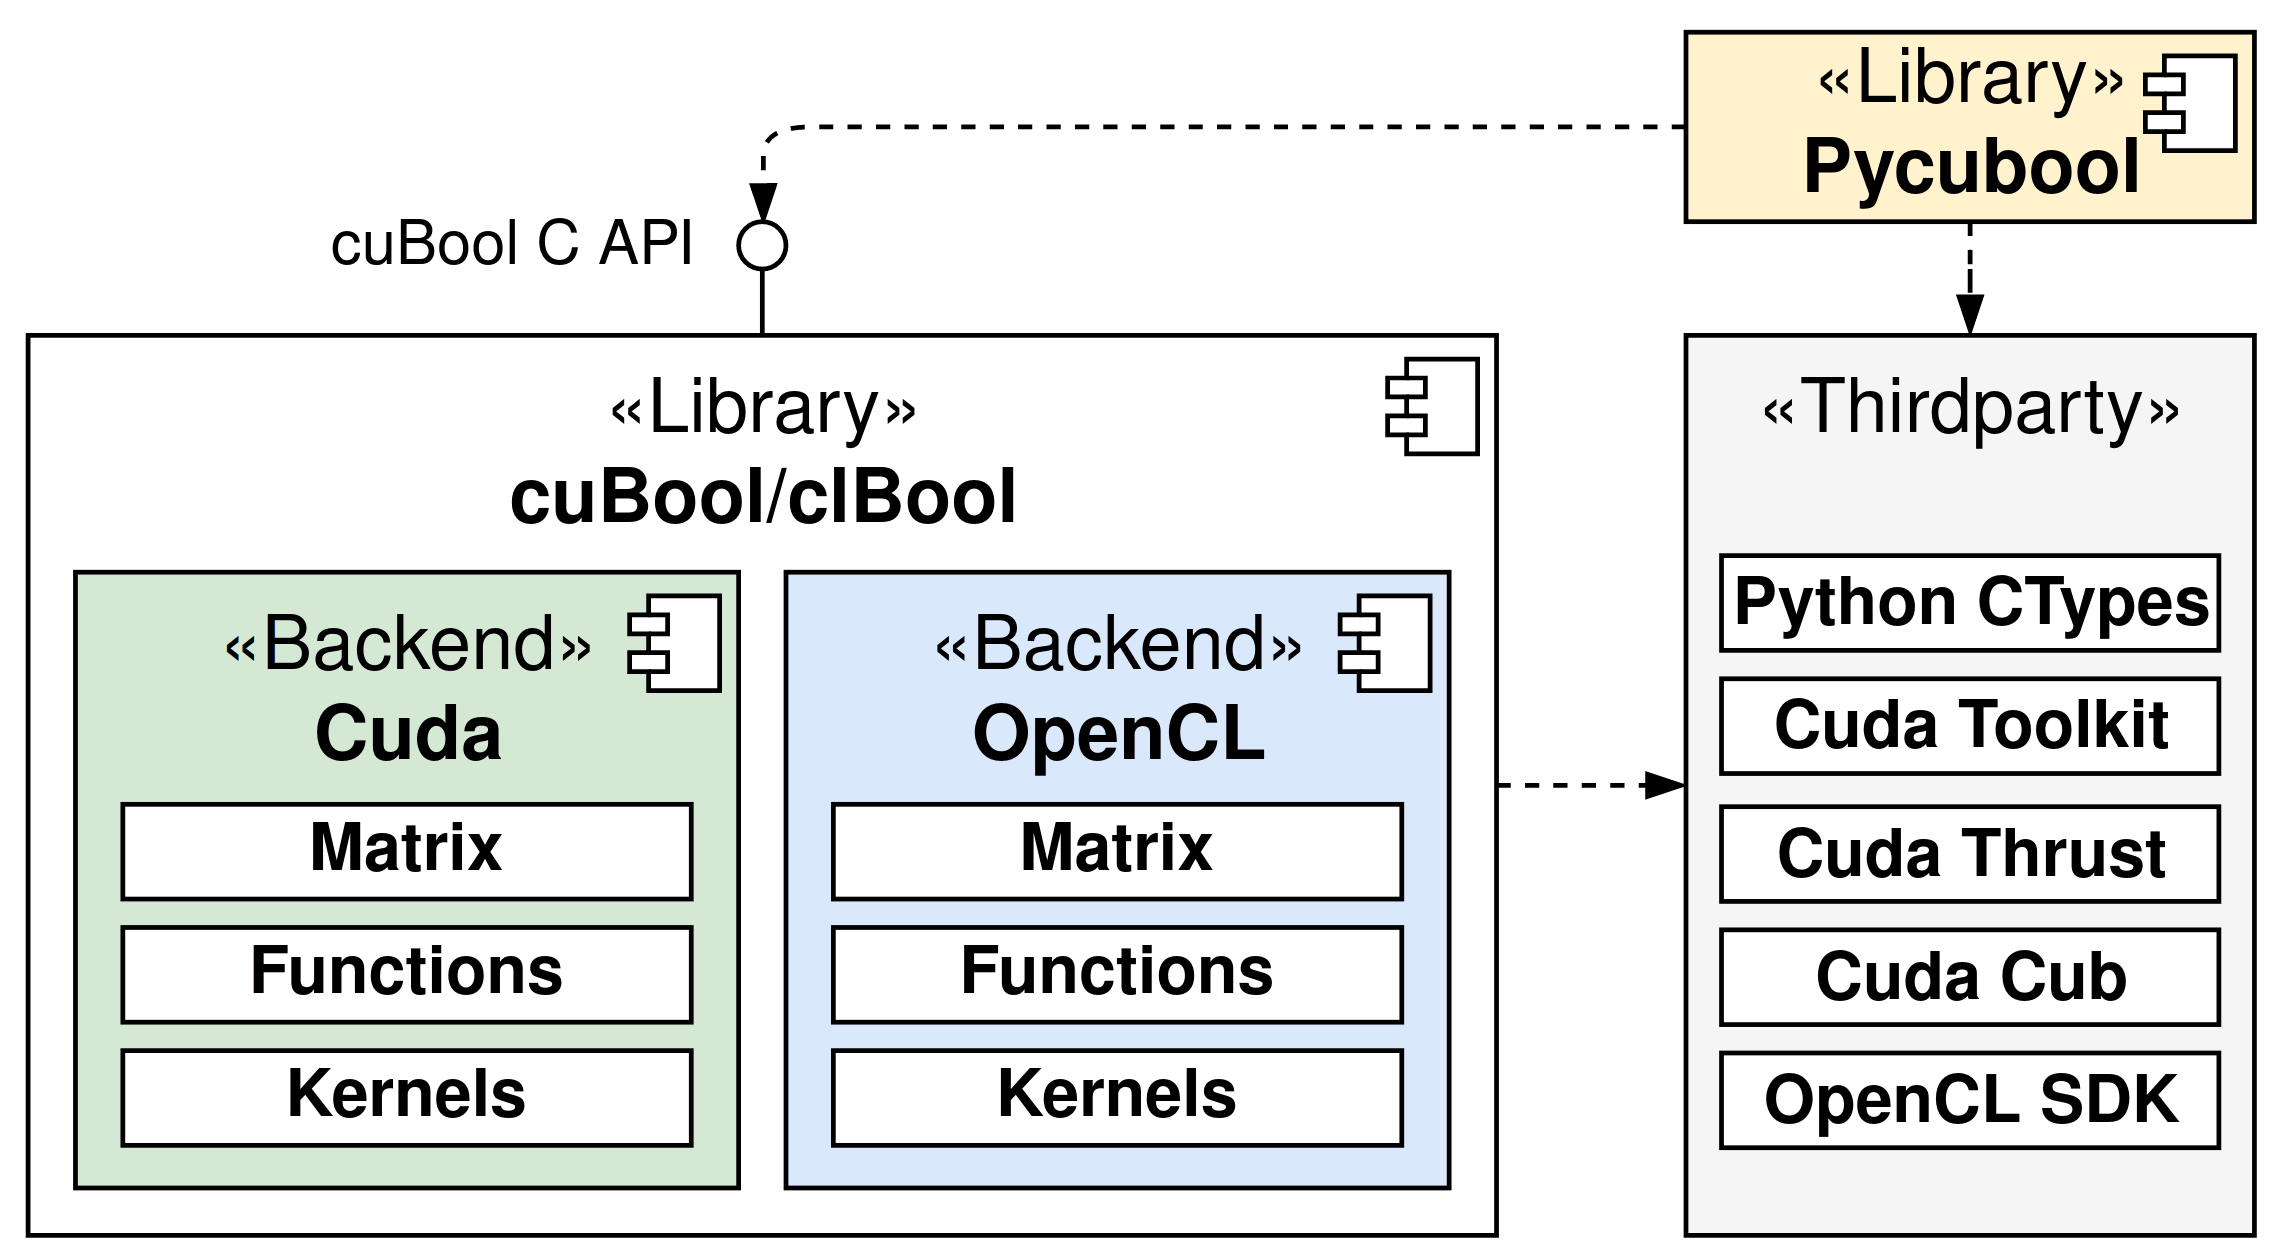
\includegraphics[width=0.39\textwidth]{generic_architecture.png}
    \caption{Sparse Boolean linear algebra library architecture.}
    \label{fig:generic_architecture}
\end{figure}

Implemented SPbLA library backends for NVIDIA Cuda and OpenCL platforms are called \textit{cuBool} and  \textit{clBool} respectively.
%%%%% I think, this info is too excessive. If you want to know something, go to the page with repos
% The projects are hosted on GitHub.
% The source code is licensed under MIT license.
% The build process is straightforward: it is configured with CMake tool and requires extra setup only for platform-specific development kits.
The general architecture of the SPbLA is depicted in figure~\ref{fig:generic_architecture}.
The core of the library is written in the C++ programming language, which is well-suited for performance and resource critical computational tasks.
The GPU related logic is in the platform specific backends.
% The GPU related logic is in the platform specific backends: Cuda and OpenCL, which use respective technologies for resources and GPU executable code management.
The library exposes C compatible API, which gives expressiveness and allows one to embed that API into other execution environments by interoperability mechanisms.
Pyspbla package encapsulates such functionality and provides it for the high-level Python runtime.

It is worth to mention, that the library is still being worked on. At this time clBool and cuBool are distinct backends, but they will be integrated into a single library.
This integration is planned for the near future.
This process requires careful selection of the interface to allow the end user to properly configure the library for specific tasks, as well as to provide the option to automatically select a specific implementation depending on the capabilities of the target device. 

However, cuBool already provides all the functionality described in the figure~\ref{fig:generic_architecture}.
It has a C compatible API, multiple backends for Cuda and CPU computations, a Python wrapper, and it is the lightweight version of the SPbLA without OpenCL computations.

Library operates on the boolean semiring with values set \{\textit{true}, \textit{false}\} with \textit{false} as an identity element, '$+$' operation is defined as logical \textit{or} and '$\times$' is defined as logical \textit{and}.
Values are also denoted as $\{1,~0\}$ respectively, and the abbreviation $\textit{nnz(M)}$ gives the number of non-zero cells of the matrix $M$.

The main primitive is a sparse matrix of boolean values, stored in one of the sparse formats.
The sparse vector is partially presented. 
Its full support will be added in the future. 
All available operations and functions are the following.

% \begin{itemize}
%     \item Create sparse matrix $M$ of size $m \times n$.
%     \item Delete sparse matrix $M$ and free all its internal resources.
%     \item Fill the matrix $M$ with values $L = \{(i,j)_k\}_k$. The result of this operation is $M_{i,j} = 1$ for each $(i, j) \in L$, and $M_{i,j} = 0$ otherwise.
%     \item \cho{Read matrix $M$ values $L = \{(i, j)~|~M_{i,j} = 1\}$.}
%     \item Matrix-matrix multiply-add operation $C \mathrel{+}= M \times N$.
%     \item Matrix-matrix add operation $M \mathrel{+}= N$.
%     \item Matrix-matrix Kronecker product $K = M \otimes N$.
% \end{itemize}

\begin{itemize}
    \item Create sparse matrix $M$ of size $m \times n$.
    \item Delete sparse matrix $M$.
    \item Fill matrix with values $\{(i,j)_k\}_k$.
    \item Read matrix values $\{(i, j)~|~M_{i,j} = 1\}$.
    \item Transpose $M = N^T$.
    \item Sub-matrix extraction $M = N[i..m, j..n]$.
    \item Matrix to vector reduce $V = \textit{reduceToColumn}(M)$.
    \item Matrix-matrix multiplication $C \mathrel{+}= M \times N$.
    \item Matrix-matrix element-wise addition $M \mathrel{+}= N$.
    \item Matrix-matrix Kronecker product $K = M \otimes N$.
\end{itemize}
\section{Implementation Details}

In this section we discuss the particular implementation details of the proposed libraries. Although general and architectural specifics are similar, the actual internal storage formats and algorithms are different. With this development strategy we address the potential problem of processing the sparse data with different values distribution, as well as the problem of proper balancing between time of the execution and memory consumption. 

\subsection{cuBool}

cuBool is sparse boolean linear algebra implementation specifically for NVIDIA Cuda platform. Core of this 
library relies on Cuda C/C++ language and API, what with NVCC compiler allows intermix C++ with Cuda 
specifics. Also cuBool employs NVIDIA Thrust auxiliary library, which provides 
implementation for generic data containers and operations, such as \textit{iterating}, \textit{exclusive or 
inclusive scan}, \textit{map} and etc., which are executed on Cuda device. That allows express algorithms in 
terms of high-level optimised primitives, what increases code readability and reduces time for development.

Sparse matrix primitive is stored in the \textit{compressed sparse row} (CSR) format with only two arrays: 
$rowspt$ for row offset indices and $cols$ for columns indices. Boolean matrices has no actual values, thus 
$true$ values are encoded only as $(i, j)$ pairs. It allows to store matrix $M$ of size $m \times n$ 
in $(m + \textit{NNZ(M)}) \times \textit{sizeof(IndexType)}$ bytes of GPU memory, where 
\textit{IndexType} is type of stored indices, for simplicity can be selected as \textit{uint32\_t}.

The algorithm Nspasrse~\cite{inproceedings:cfpq_for_redis_graph} is used for matrix-matrix multiplication. 
This algorithm is a boolean values case 
adaptation of the state-of-the-art, efficient and memory saving sparse general matrix multiplication (SpGEMM) 
algorithm, proposed in Yusuke Nagasaka et al. research~\cite{algo:spgemm:8025284}. This algorithm was selected because it 
gives promising relatively small memory footprint for large matrices processing, as well as it competes with 
other major Cuda SpGEMM implementations, such as cuSPARSE or CUSP.  

Matrix-matrix addition is based on GPU Merge Path algorithm~\cite{inproceedings:gpu_merge_path} with 
dynamic work balancing and two pass processing. 
These optimizations give better workload dispatch among execution blocks and allow more precise memory allocations in
order to keep memory footprint small respectively. 

As an example of library C API embedding, cuBool provides python wrapper, called Pycubool. This module exports 
library functionality via default CTypes module for native functions calling and provides safe and automated 
management for native resources. 

\subsection{clBool}

clBool is sparse boolean linear algebra implementation for OpenCL platform. This library is implemented 
in the C++ with OpenCL kernels, stored as separate source files, loaded on demand at runtime. 

Sparse matrix primitive is stored in \textit{coordinate format} (COO) with two arrays: $rows$ and $cols$ 
for row and column indices of the stored non-zero values. For the matrix $M$ of size $m \times n$ memory 
consumption is $2 \times \textit{NNZ(M)} \times \textit{sizeof(IndexType)}$. This format was selected 
instead of CSR, because COO gives better memory footprint for very sparse matrices with a lot of empty rows.

\textbf{!!! Matrix-matrix multiplication !!!}

Matrix-matrix addition is based on GPU Merge Path algorithm as well. Since all COO matrix values are stored in 
the single array, its merge can be completed at single time, compared to CSR matrix merge computed on a 
per row basis. This operation is implemented in a classic one pass fashion: it allocates single merge 
buffer of size $\textit{NNZ(A)} + \textit{NNZ(B)})$ before actual merge of matrices $A$ and $B$, what can
negatively affect memory consumption for large matrices with lots of duplicated non-zero values at the 
same positions.

\textbf{!!! Something about managed environment wrapper !!!}

\section{Evaluation}

The goal of this evaluation is to investigate the applicability of the proposed algorithm to both regular and context-free path querying.
We measured the execution time of the index creation which solves the reachability problem for both kinds of queries.
The execution time for CFPQ was compared with the Azimov's algorithm for CFPQ reachability.
We also investigated the practical applicability of paths extraction algorithm to both regular and context-free path queries.

For evaluation, we used a PC with Ubuntu 18.04 installed.
It has Intel core i7-6700 CPU, 3.4GHz, and DDR4 64Gb RAM.
We only measure the execution time of the algorithms themselves, thus we assume an input graph is loaded into RAM in the form of its adjacency matrix in the sparse format.
Note, that the time needed to load an input graph into the RAM is excluded from the time measurements.

\subsection{RPQ Evaluation}

To investigate the applicability of the proposed algorithm for regular path querying we gathered a dataset which consists of both real-world and synthetically generated graphs.
We generated the queries from the most popular RPQ templates.

\subsubsection{Dataset}

We gathered several graphs which represent real-world data from different areas and are frequently used for evaluation of the graph querying algorithms.
Namely, the dataset consists of three parts.
The first part is the set of LUBM graphs\footnote{Lehigh University Benchmark (LUBM) web page: \url{http://swat.cse.lehigh.edu/projects/lubm/}. Access date: 07.07.2020.}~\citep{10.1016/j.websem.2005.06.005} which have different numbers of vertices.
The second one is the set of graphs from Uniprot database\footnote{Universal Protein Resource (UniProt) web page: \url{https://www.uniprot.org/}. All files used can be downloaded via the link: \url{ftp://ftp.uniprot.org/pub/databases/uniprot/current_release/rdf/}. Access date: 07.07.2020.}: \textit{proteomes}, \textit{taxonomy} and \textit{uniprotkb}.
The~last part consists of the RDF files \textit{mappingbased\_properties} from DBpedia\footnote{DBpedia project web site: \url{https://wiki.dbpedia.org/}. Access date: 07.07.2020.} and \textit{geospecies}\footnote{The Geospecies RDF: \url{https://old.datahub.io/dataset/geospecies}. Access date: 07.07.2020.}.
A brief description of the graphs in the dataset is presented in Table~\ref{tbl:graphs_for_rpq}.

\begin{table}
    \centering
\caption{Graphs for RPQ evaluation}
\label{tbl:graphs_for_rpq}
{

\rowcolors{2}{black!2}{black!10}
\begin{tabular}{|l|c|c|}
\hline
Graph & \#V & \#E  \\
\hline
\hline
LUBM1k  & 120 926 & 484 646 \\
LUBM3.5k  & 358 434 & 144 9711 \\
LUBM5.9k  & 596 760 & 2 416 513 \\
LUBM1M   & 1 188 340 & 4 820 728 \\
LUBM1.7M & 1 780 956 & 7 228 358 \\
LUBM2.3M & 2 308 385 & 9 369 511 \\
\hline
Uniprotkb & 6 442 630 & 24 465 430 \\
Proteomes & 4 834 262 & 12 366 973 \\
Taxonomy & 5 728 398 & 14 922 125 \\
\hline
Geospecies & 450 609 & 2 201 532 \\
Mappingbased\_properties & 8 332 233 & 25 346 359 \\
\hline
\end{tabular}
}
\end{table}


Queries for evaluation were generated from the templates for the most popular RPQs, specifically the queries presented in Table 2 in~\cite{Pacaci2020RegularPQ} and in Table 5 in~\cite{Wang2019}.
These query templates are presented in Table~\ref{tbl:queries_templates}.
We generate 10 queries for each template and each graph.
The most frequent relations from the given graph were used as symbols in the query template\footnote{Used generator is available as part of CFPQ\_data project: \url{https://github.com/JetBrains-Research/CFPQ_Data/blob/master/tools/gen_RPQ/gen.py}. Access data: 07.07.2020.}.
We used the same set of queries for all LUBM graphs to investigate scalability of the proposed algorithm.

\begin{table}
    \centering
\caption{Queries templates for RPQ evaluation}
\label{tbl:queries_templates}
{\small
\renewcommand{\arraystretch}{1.2}
\rowcolors{2}{black!2}{black!10}
\begin{tabular}{|c|c||c|c|}
\hline

Name & Query & Name & Query \\
\hline
\hline
$Q_1$   & $a^*$                               & $Q_9^5$    & $(a \mid b \mid c \mid d \mid e)^+$                     \\
$Q_2$   & $a\cdot b^*$                        & $Q_{10}^2$ & $(a \mid b) \cdot c^*$                                  \\
$Q_3$   & $a \cdot b^* \cdot c^*$             & $Q_{10}^3$ & $(a \mid b \mid c)  \cdot d^*$                          \\
$Q_4^2$ & $(a \mid b)^*$                      & $Q_{10}^4$ & $(a \mid b \mid c \mid d)  \cdot e^*$                   \\
$Q_4^3$ & $(a \mid b \mid c)^*$               & $Q_{10}^5$ & $(a \mid b \mid c \mid d \mid e)  \cdot f^*$            \\
$Q_4^4$ & $(a \mid b \mid c \mid d)^*$        & $Q_{10}^2$ & $a \cdot b$                                             \\
$Q_4^5$ & $(a \mid b \mid c \mid d \mid e)^*$ & $Q_{11}^3$ & $a \cdot b \cdot c$                                     \\
$Q_5$   & $a \cdot b^* \cdot c$               & $Q_{11}^4$ & $a \cdot b \cdot c \cdot d$                             \\
$Q_6$   & $a^* \cdot b^*$                     & $Q_{11}^5$ & $a \cdot b \cdot c \cdot d \cdot f$                     \\
$Q_7$   & $a \cdot b \cdot c^*$               & $Q_{12}$   & $(a \cdot b)^+ \mid  (c \cdot d)^+$                     \\
$Q_8$   & $a? \cdot b^*$                      & $Q_{13}$   & $(a \cdot(b \cdot c)^*)^+ \mid  (d \cdot f)^+$          \\
$Q_9^2$ & $(a \mid b)^+$                      & $Q_{14}$   & $(a \cdot b \cdot (c \cdot d)^*)^+  \cdot (e \mid f)^*$ \\
$Q_9^3$ & $(a \mid b \mid c)^+$               & $Q_{15}$   & $(a \mid b)^+ \cdot (c \mid d)^+$                       \\
$Q_9^4$ & $(a \mid b \mid c \mid d)^+$        & $Q_{16}$   & $a \cdot b \cdot (c \mid d \mid e)$                     \\
\hline
\end{tabular}
}
\end{table}


\subsubsection{Results}

We averaged the execution time of index creation over 5 runs for each query.
Index creation time for LUBM graphs set is presented in Figure~\ref{fig:lubm_all_qs}.
We can see that evaluation time depends on the query: there are queries which evaluate in less than 1 second even for the largest graphs ($Q_2$, $Q_5$, $Q_{11}^2$, $Q_{11}^3$), while the worst time is 6.26 seconds ($Q_{14}$).
The execution time of our algorithm is comparable with the recent results for the same graphs and queries implemented on a distributed system over 10 nodes~\citep{Wang2019}, while we use only one node.
We conclude that our algorithm demonstrates reasonable performance to be applied to the real-world data analysis.
%\cho{Note that the accurate comparison of different approaches may be a promising direction of future research.}

\begin{figure}
    \centering
   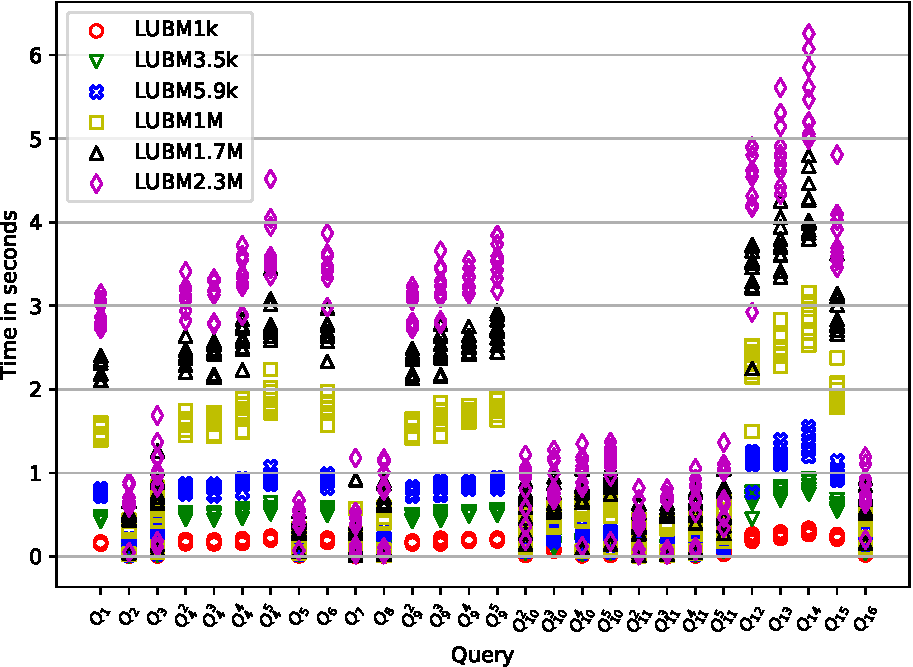
\includegraphics[width=0.6\textwidth]{data/LUBM_all.pdf}
   \caption{Index creation time for LUBM graphs}
   \label{fig:lubm_all_qs}
\end{figure}

Index creation time for each query on the real-world graphs is presented in Figure~\ref{fig:other_all_qs}.
We can see that querying small graphs requires more time than querying bigger graphs in some cases.
For example, conseder $Q_{10}^4$: querying the \textit{geospecies} graph (450k vertices) in some cases requires more time than querying of \textit{mappingbased\_properties} (8.3M vertices) and \textit{taxonomy} (5.7M vertices).
We conclude that the evaluation time depends on the inner structure of a graph.
On the other hand, \textit{taxonomy} querying in many cases requires significantly more time than for other graphs, while \textit{taxonomy} is not the biggest graph.
Finally, in most cases query execution lasts less than 10 seconds, even for bigger graphs, and no query requires more than 52.17 seconds.

\begin{figure}
    \centering
   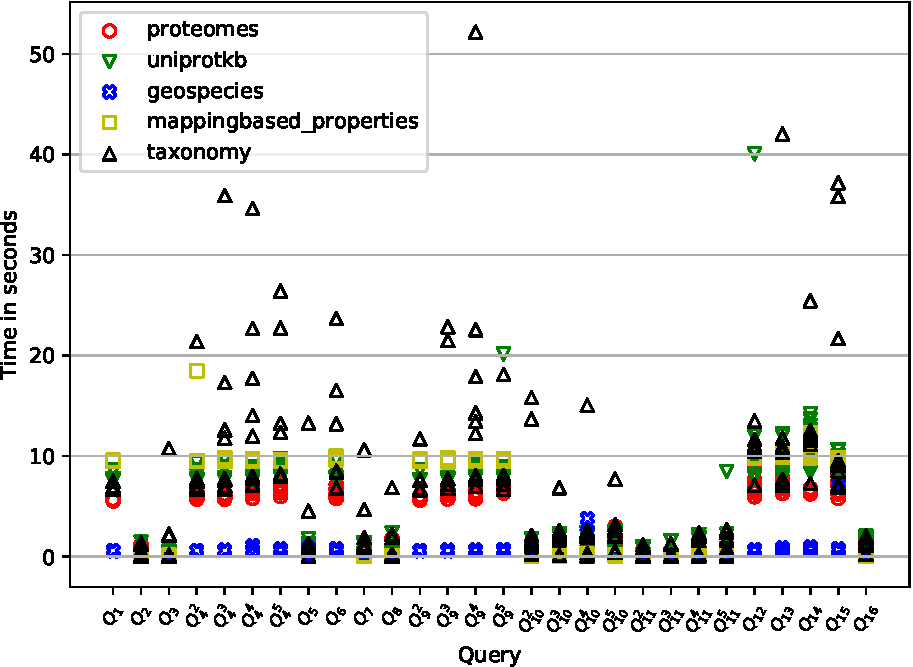
\includegraphics[width=0.6\textwidth]{data/other_all.pdf}
   \caption{Index creation time for real-world RDFs}
   \label{fig:other_all_qs}
\end{figure}

%We evaluate path extraction for queries which result in possibly long paths.
%Long paths usually require many iterations of transitive closure evaluation, thus we used the number of the iterations as a criterion to select the inputs for the evaluation.
%For each selected graph and query we measure paths extraction time for each reachable pair.
%Since the index can be reused from the previous step, we omit the time necessary to create the index.
%We limit by 10 the number of paths to extract.

%In Figures~\ref{fig:geo_tensors_rpq} and~\ref{fig:dbpedia_tensors_rpq} we show the time needed to extract a path of a specific length when only one path was extracted.
%The main observation is that time is linear on the path length, even if a generic path extraction procedure is used.

%\begin{figure}
%     \begin{subfigure}[b]{0.45\textwidth}
%         \centering
%         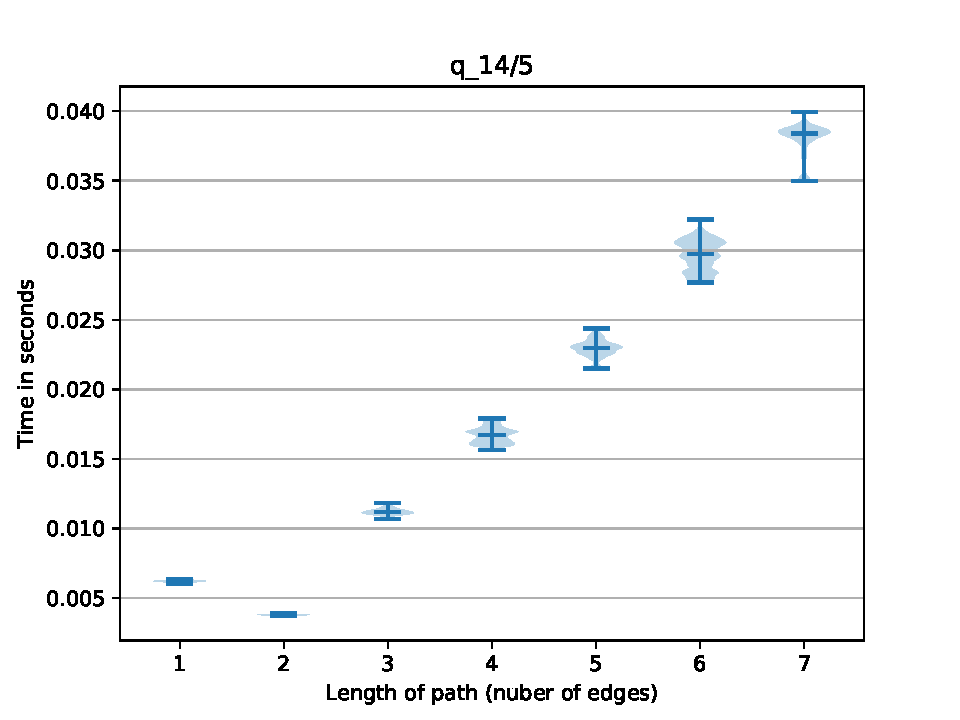
\includegraphics[width=\textwidth]{../paper/data/geo_rpq_single_path/q_14_5.pdf}
%         \caption{\footnotesize \textit{geospecies}, $Q_{14}$}
%         \label{fig:geo_tensors_rpq}
%     \end{subfigure}
%     ~\begin{subfigure}[b]{0.45\textwidth}
%         \centering
%         \includegraphics[width=\textwidth]{../paper/data/CF/Tensor_path/dbpedia_path_tensor.pdf}
%         \caption{\footnotesize \textit{mappingbased\_properties}, $Q_{4}^5$}
%         \label{fig:dbpedia_tensors_rpq}
%     \end{subfigure}\\
%     \begin{subfigure}[b]{0.45\textwidth}
%         \centering
%         \includegraphics[width=\textwidth]{../paper/data/CF/Matrix_CF/geo_path_matrix.pdf}
%         \caption{\footnotesize \textit{geospecies}, \textit{Geo}}
%         \label{fig:geo_matrix_cfpq}
%     \end{subfigure}
%     ~\begin{subfigure}[b]{0.45\textwidth}
%         \centering
%         \includegraphics[width=\textwidth]{../paper/data/CF/Tensor_path/geo_path_tensor.pdf}
%         \caption{\footnotesize \textit{geospecies}, \textit{Geo}}
%         \label{fig:geo_tensors_cfpq}
%     \end{subfigure}\\
%   \caption{Single path extraction for specific graph and query for our solution (\subref{fig:geo_tensors_rpq}, \%subref{fig:dbpedia_tensors_rpq}, \subref{fig:geo_tensors_cfpq}), and Azimov's (\subref{fig:geo_matrix_cfpq})}
%\end{figure}

\subsection{CFPQ Evaluation}

We evaluate the applicability of the proposed algorithm to CFPQ processing over real-world graphs on a number of classic cases and compare them with the Azimov's algorithm.
Currently only a single path version of Azimov's algorithm exists, and we use its implementation using PyGraphBLAS. Note that it is not trivial to compare our results with the state-of-the-art results provided by~\cite{10.1145/3398682.3399163} (Azimov's algorithm) because our algorithm computes significantly more information. While the state-of-the-art solution computes only reachability facts or a single-path semantics, our algorithm computes data necessary to restore all possible paths.

\subsubsection{Dataset}

We use CFPQ\_Data\footnote{CFPQ\_Data is a dataset for CFPQ evaluation which contains both synthetic and real-world data and queries \url{https://github.com/JetBrains-Research/CFPQ\_Data}. Access date: 07.07.2020.} dataset for evaluation.
Namely, we use relatively big RDF files and respective same-generation queries $G_1$~(Eq.~\ref{eqn:g_1}) and $G_2$~(Eq.~\ref{eqn:g_2}) which are used in other works for CFPQ evaluation.
We also use the $Geo$~(Eq.~\ref{eqn:geo}) query provided by~\cite{Kuijpers:2019:ESC:3335783.3335791} for \textit{geospecies} RDF.
Note that we use $\overline{x}$ notation in queries to denote the inverse of $x$ relation and the respective edge.
\begin{align}
\begin{split}
\label{eqn:g_1}
S \to & \overline{\textit{subClassOf}} \ \ S \ \textit{subClasOf} \mid \overline{\textit{type}} \ \ S \ \textit{type}\\   & \mid \overline{\textit{subClassOf}} \ \ \textit{subClasOf} \mid \overline{\textit{type}} \ \textit{type}
\end{split}
\end{align}
\begin{align}
\begin{split}
\label{eqn:g_2}
S \to \overline{\textit{subClassOf}} \ \ S \ \textit{subClasOf} \mid \textit{subClassOf}
\end{split}
\end{align}
\begin{align}
\begin{split}
\label{eqn:geo}
S \to & \textit{broaderTransitive} \ \  S \ \overline{\textit{broaderTransitive}} \\
      & \mid \textit{broaderTransitive} \ \  \overline{\textit{broaderTransitive}}
\end{split}
\end{align}
\begin{align}
\begin{split}
\label{eqn:ma}
S & \to \overline{d} \ V \ d \\
V & \to ((S?) \overline{a})^* (S?) (a (S?))^*
\end{split}
\end{align}

Additionally we evaluate our algorithm on memory aliases analysis problem: a well-known problem which can be reduced to CFPQ~\citep{Zheng:2008:DAA:1328897.1328464}.
To do it, we use some graphs built for different parts of Linux OS kernel (\textit{arch}, \textit{crypto}, \textit{drivers}, \textit{fs}) and the query $MA$~(Eq.~\ref{eqn:ma})~\citep{10.1145/3093336.3037744}.
The detailed data about all the graphs used is presented in Table~\ref{tbl:graphs_for_cfpq}.

{\setlength{\tabcolsep}{0.3em}
\begin{table}
    \centering
{
\caption{Graphs for CFPQ evaluation: \textit{bt} is broaderTransitive, \textit{sco} is subCalssOf}
\label{tbl:graphs_for_cfpq}
\scriptsize
\rowcolors{2}{black!2}{black!10}
\begin{tabular}{|l|c|c|c|c|c|c|c|}
\hline
Graph          & \#V       & \#E        & \#sco & \#type &\#bt & \#a  & \#d \\
\hline
\hline
eclass\_514en  & 239 111    & 523 727    & 90 512    & 72 517    &        ---        & ---  & --- \\
enzyme         & 48 815     & 109 695    & 8 163     & 14 989    &        ---        & ---  & --- \\
geospecies     & 450 609    & 2 201 532  & 0         & 89 062    &        20 867     & ---  & --- \\
go             & 272 770    & 534 311    & 90 512    & 58 483    &        ---        & ---  & --- \\
go-hierarchy   & 45 007     & 980 218    & 490 109   & 0         &        ---        & ---  & --- \\
taxonomy       & 5 728 398  & 14 922 125 & 2 112 637 & 2 508 635 &        ---        & ---  & --- \\
\hline
arch           & 3 448 422  & 5 940 484  &      ---     &  ---   &        ---        & 671 295 & 2 298 947 \\
crypto         & 3 464 970  & 5 976 774  &      ---     &  ---   &        ---        & 678 408 & 2 309 979 \\
drivers        & 4 273 803  & 7 415 538  &      ---     &  ---   &        ---        & 858 568 & 2 849 201 \\
fs             & 4 177 416  & 7 218 746  &      ---     &  ---   &        ---        & 824 430 & 2 784 943 \\
\hline
\end{tabular}
}
\end{table}
}
\subsubsection{Results}

We averaged the index creation time over 5 runs for both single-path Azimov's algorithm (\textbf{Mtx}) and the proposed algorithm (\textbf{Tns}) (see Table~\ref{tbl:CFPQ_index}).

{\setlength{\tabcolsep}{0.2em}
  \begin{table}
    \centering
    \caption{CFPQ evaluation results, time is measured in seconds}
    \label{tbl:CFPQ_index}
    \rowcolors{4}{black!2}{black!10}
    \small
    \begin{tabular}{| l | c | c | c | c | c | c | c | c |}
      \hline

      \multirow{2}{*}{Name}  & \multicolumn{2}{c|}{$G_1$} & \multicolumn{2}{c|}{$G_2$} & \multicolumn{2}{c|}{\textit{Geo}} & \multicolumn{2}{c|}{\textit{MA}}\\
      \cline{2-9}
                      & Tns    & Mtx    & Tns  & Mtx  & Tns   & Mtx   & Tns     & Mtx \\
      \hline
      \hline
      eclass\_514en   & 0.24   & 0.27   & 0.25 & 0.26 & ---   & ---   & ---     & ---\\
      enzyme          & 0.03   & 0.04   & 0.02 & 0.01 & ---   & ---   & ---     & ---\\
      geospecies      & 0.08   & 0.06   & $0^{*}$ & 0.01 & 26.12 & 16.58 & ---     & ---\\
      go-hierarchy    & 0.16   & 1.43   & 0.23 & 0.86 & ---   & ---   & ---     & ---\\
      go              & 1.56   & 1.74   & 1.21 & 1.14 & ---   & ---   & ---     & ---\\
      pathways        & 0.01   & 0.01   & 0.01 & 0.01 & ---   & ---   & ---     & ---\\
      taxonomy        & 4.81   & 2.71   & 3.75 & 1.56 & ---   & ---   & ---     & ---\\
      \hline
      arch            & ---    & ---    & ---  & ---  & ---   & ---   & 262.45  & 195.51  \\
      crypto          & ---    & ---    & ---  & ---  & ---   & ---   & 267.52  & 195.54  \\
      drivers         & ---    & ---    & ---  & ---  & ---   & ---   & 1309.57 & 1050.78 \\
      fs              & ---    & ---    & ---  & ---  & ---   & ---   & 470.49  & 370.73  \\
      \hline
    \end{tabular}
  \end{table}
}

Best to our knowledge, the proposed algorithm is the first algorithm that provides information about all paths of interest (Azimov's algorithm computes information about only one path).
The direct comparison with other solutions is impossible, and we just estimate the running time of our algorithm for a small number of cases.
Namely, we extract all paths with length not greater than 20 edges between all pairs of vertices from indeces created for graphs \textit{go} and \textit{eclass\_514en} and query $G_1$.
Paths extraction for one pair of vertices requires 2.64 seconds averaged over all pairs for \textit{go} graph. The~maximal time is 4699 seconds and 217737 paths were extracted during this time. The average number of paths between two vertices is 184.
For \textit{eclass\_514en} paths extraction for one pair of vertices requires 1.27 seconds averaged over all pairs. The~maximal time is 8.04 seconds and only one path is extracted during this time. The average number of paths between two vertices is 3.
We can see that paths can be extracted in a reasonable time, but a detailed analysis of paths extraction algorithm performance depends on graphs structure.

%Comparison of paths extraction is presented in Figures~\ref{fig:geo_matrix_cfpq} and~\ref{fig:geo_tensors_cfpq}.
%While both methods demonstrate linear time on the length of the extracted path, our generic solution is more than 1000 times slower than Azimov's single path extraction procedure.
%We conclude that current generic all-path extraction procedure is not optimal for single path extraction.

\subsection{Conclusion}

We conclude that the proposed algorithm is applicable to real-world data processing: the algorithm allows one to solve both the reachability problem and to extract paths of interest in a reasonable time even using naive implementation.
While index creation time (reachability query evaluation) is comparable with other existing solutions, paths extraction procedure should be improved in the future. However, the state-of-the-art solution computes only reachability facts or a single-path semantics, whereas our algorithm computes data necessary to restore all possible paths (all-paths semantics).
Finally, a detailed comparison of the proposed solution with other algorithms for CFPQ and RPQ is required.

To summarize the overall evaluation, the proposed algorithm is applicable to both RPQ and CFPQ over real-world graphs.
Thus, the proposed solution is a promising unified algorithm for both RPQ and CFPQ evaluation.

\section{Conclusion}

Conclusion, current state, results.

Future work. Library extension up to full GraphBLAS API implementation.

LaGraph on F\# .NET.

Evaluation. Comparison with other implementations on different devices.
Manual implementation versus translation.  

Another direction of future work is Brahma.FSharp improvements. 
First of all, it is necessary to support discriminated unions to make it possible to express custom semirings such as \texttt{Min-Plus}, as presented in listing~\ref{lst_example}. 

Also, it is necessary to add high-level abstractions for asynchronous programming, and for multi-GPU programming.
Such mechanisms can be naturally expressed in F\# with native primitives for asynchronous programming.

fusion and other optimizations.
\begin{frame}
    \frametitle{Ответы на замечания ведущей организации НИИ~<<Рога~и~копыта>>}
    \begin{itemize}
        \item Замечание -- ответ
        \item Замечание -- ответ
        \item Замечание -- ответ
        \item Замечание -- ответ
        \item Замечание -- ответ
    \end{itemize}
\end{frame}

\begin{frame}
    \frametitle{Ответы на замечания оф. оппонента Иванова\,И.\,И}
    \begin{itemize}
        \item Замечание -- ответ
        \item Замечание -- ответ
        \item Замечание -- ответ
        \item Замечание -- ответ
        \item Замечание -- ответ
    \end{itemize}
\end{frame}

\begin{frame}
    \frametitle{Ответы на замечания Петрова\,П.\,П}
    \begin{itemize}
        \item Замечание -- ответ
        \item Замечание -- ответ
        \item Замечание -- ответ
        \item Замечание -- ответ
        \item Замечание -- ответ
    \end{itemize}
\end{frame}


%\section*{Acknowledgment}
%
%The preferred spelling of the word ``acknowledgment'' in America is without
%an ``e'' after the ``g''. Avoid the stilted expression ``one of us (R. B.
%G.) thanks $\ldots$''. Instead, try ``R. B. G. thanks$\ldots$''. Put sponsor
%acknowledgments in the unnumbered footnote on the first page.


\bibliographystyle{./IEEEtran}
\bibliography{./Sparse_Boolean_Algebra_on_GPGPU}

\end{document}
